\documentclass[tikz,convert={outfile=images/ping-pong-0.png,density=1000}]{standalone}
\usepackage[build={latexoptions={-output-directory=latex/png}}]{standalone}
\usetikzlibrary{automata, positioning, arrows}
\usepackage{xcolor}
\newcommand{\StIdle}{\tiny\texttt{StIdle}}
\newcommand{\StBusy}{\tiny\texttt{StBusy}}
\newcommand{\StDone}{\tiny\texttt{StDone}}
\newcommand{\MsgPing}{\tiny\texttt{MsgPing}}
\newcommand{\MsgPong}{\tiny\texttt{MsgPong}}
\newcommand{\MsgDone}{\tiny\texttt{MsgDone}}
\newcommand{\StIdleX}{\tiny\texttt{StIdle2}}
\newcommand{\StBusyX}{\tiny\texttt{StBusy2}}
\newcommand{\StDoneX}{\tiny\texttt{StDone2}}
\newcommand{\MsgPingX}{\tiny\texttt{MsgPing2}}
\newcommand{\MsgPongX}{\tiny\texttt{MsgPong2}}
\newcommand{\MsgBusy}{\tiny\texttt{MsgBusy}}
\newcommand{\MsgDoneX}{\tiny\texttt{MsgDone2}}
\definecolor{mygreen}{rgb}{0.109804,0.698039,0.341176}
\definecolor{myblue}{rgb}{0.360784,0.423529,255}
\begin{document}
\tikzset{
    state/.style={
           rectangle,
           draw=white!40!black,
           minimum height=1em,
           inner sep=1pt,
           text centered
           },
    ->/.style={draw=white!40!black,-stealth}
}
\tikzstyle{every node}=[color=white!40!black,font=\tiny]

% PingPong, v1
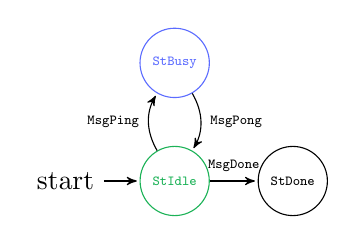
\begin{tikzpicture}[->,>=stealth',shorten >=1pt,auto,node distance=1.5cm]
  \node[state, mygreen, initial]      (Idle) {\StIdle};
  \node[state, right of=Idle]         (Done) {\StDone};
  \node[state, myblue, above of=Idle] (Busy) {\StBusy};

  \draw (Idle) edge[above]            node{\MsgDone} (Done);
  \draw (Idle) edge[left, bend left]  node{\MsgPing} (Busy);
  \draw (Busy) edge[right, bend left] node{\MsgPong} (Idle);
\end{tikzpicture}
\end{document}

